\documentclass{article}
\usepackage{v-test-paper}
\title{\textsc{JEE Advanced 2021 Paper-I\\Physics}}
\newenvironment{solution}{\par\noindent\color{red!85!black}$\Rightarrow$\vspace{0em}}{}
\date{}
\begin{document}
\maketitle


\begin{enumerate}
    \item The smallest division on the main scale of a Vernier calipers is 0.1 cm. Ten divisions of the Vernier scale correspond to nine divisions of the main scale. The figure below on the left shows the reading of this calipers with no gap between its two jaws. The figure on the right shows the reading with a solid sphere held between the jaws. The correct diameter of the sphere is
    \begin{center}
        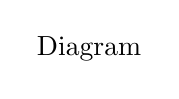
\begin{tikzpicture}
        \node {Diagram};
        \end{tikzpicture}
        \end{center}
        \begin{tasks}(2)
            	\task 3.07 cm
            	\task 3.11 cm
            	\task 3.15 cm
            	\task 3.17 cm
        \end{tasks}
    \item An ideal gas undergoes a four step cycle as shown in the \(P - V\) diagram below. During this cycle, heat is absorbed by the gas in
    \begin{center}
        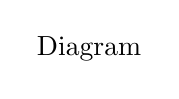
\begin{tikzpicture}
        \node {Diagram};
        \end{tikzpicture}
        \end{center}
        \begin{tasks}(2)
            	\task steps 1 and 2
            	\task steps 1 and 3
            	\task steps 1 and 4
            	\task steps 2 and 4
        \end{tasks}

    \item An extended object is placed at point O, 10 cm in front of a convex lens \(L_1\) and a concave lens \(L_2\) is placed 10 cm behind it, as shown in the figure. The radii of curvature of all the curved surfaces in both the lenses are 20 cm. The refractive index of both the lenses is 1.5. The total magnification of this lens system is
    \begin{center}
        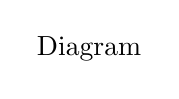
\begin{tikzpicture}
            \node {Diagram};
        \end{tikzpicture}
    \end{center}
        \begin{tasks}(2)
            \task 0.4
            \task 0.8
            \task 1.3
            \task 1.6
        \end{tasks}
        
    \item A heavy nucleus \(Q\) of half-life 20 minutes undergoes alpha-decay with probability of 60\% and beta-decay with probability of 40\%. Initially, the number of \(Q\) nuclei is 1000. The number of alpha-decays of \(Q\) in the first one hour is
        \begin{tasks}(2)
            \task 50
            \task 75
            \task 350
            \task 525
        \end{tasks}




\section*{SECTION 2}


\subsection*{Question Stem for Question Nos. 5 and 6}

\textbf{Question Stem}

A projectile is thrown from a point O on the ground at an angle $45^\circ$ from the vertical and with a speed $5\sqrt{2}$ m/s. The projectile at the highest point of its trajectory splits into two equal parts. One part falls vertically down to the ground, $0.5$ s after the splitting. The other part, $t$ seconds after the splitting, falls to the ground at a distance $x$ meters from the point O. The acceleration due to gravity $g = 10$ m/s$^2$.


    \item The value of $t$ is \_\_\_\_.
    \item The value of $x$ is \_\_\_\_.


\subsection*{Question Stem for Question Nos. 7 and 8}

\textbf{Question Stem}

In the circuit shown below, the switch S is connected to position P for a long time so that the charge on the capacitor becomes $q_1$ $\mu$C. Then S is switched to position Q. After a long time, the charge on the capacitor is $q_2$ $\mu$C.
\begin{center}
    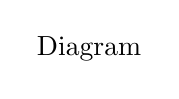
\begin{tikzpicture}
        \node {Diagram};
    \end{tikzpicture}
\end{center}

% Insert circuit diagram here (not included in LaTeX as per instructions)

    \item The magnitude of $q_1$ is \_\_\_\_.
    \item The magnitude of $q_2$ is \_\_\_\_.


\subsection*{Question Stem for Question Nos. 9 and 10}

\textbf{Question Stem}

Two point charges $-Q$ and $+Q/\sqrt{3}$ are placed in the xy-plane at the origin $(0, 0)$ and a point $(2, 0)$, respectively, as shown in the figure. This results in an equipotential circle of radius R and potential V = 0 in the xy-plane with its center at $(b, 0)$. All lengths are measured in meters.
\begin{center}
    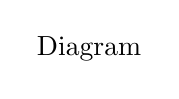
\begin{tikzpicture}
        \node {Diagram};
    \end{tikzpicture}
\end{center}

% Insert point charges and equipotential circle diagram here (not included in LaTeX as per instructions)

    \item The value of R is \_\_\_\_ meter.
    \item The value of b is \_\_\_\_ meter.

    \item A horizontal force $F$ is applied at the center of mass of a cylindrical object of mass $m$ and radius $R$, perpendicular to its axis as shown in the figure. The coefficient of friction between the object and the ground is $\mu$. The center of mass of the object has an acceleration $a$. The acceleration due to gravity is $g$. Given that the object rolls without slipping, which of the following statement(s) is(are) correct?
        \begin{tasks}(1)
            	\task For the same $F$, the value of $a$ does not depend on whether the cylinder is solid or hollow
            	\task For a solid cylinder, the maximum possible value of $a$ is $2\mu g$
            	\task The magnitude of the frictional force on the object due to the ground is always $\mu mg$
            	\task For a thin-walled hollow cylinder, $a = \frac{F}{2m}$
        \end{tasks}

    \item A wide slab consisting of two media of refractive indices $n_1$ and $n_2$ is placed in air as shown in the figure. A ray of light is incident from medium $n_1$ to $n_2$ at an angle $\theta$, where $\sin \theta$ is slightly larger than $1/n_1$. Take refractive index of air as 1. Which of the following statement(s) is(are) correct?
        \begin{tasks}(1)
            	\task The light ray enters air if $n_2 = n_1$
            	\task The light ray is finally reflected back into the medium of refractive index $n_1$ if $n_2 < n_1$
            	\task The light ray is finally reflected back into the medium of refractive index $n_1$ if $n_2 > n_1$
            	\task The light ray is reflected back into the medium of refractive index $n_1$ if $n_2 = 1$
        \end{tasks}

    \item A particle of mass $M = 0.2 \, \text{kg}$ is initially at rest in the $xy$-plane at a point $(x = -l, y = -h)$, where $l = 10 \, \text{m}$ and $h = 1 \, \text{m}$. The particle is accelerated at time $t = 0$ with a constant acceleration $a = 10 \, \text{m/s}^2$ along the positive $x$-direction. Its angular momentum and torque with respect to the origin, in SI units, are represented by $\vec{L}$ and $\vec{\tau}$, respectively. $\hat{i}$, $\hat{j}$ and $\hat{k}$ are unit vectors along the positive $x$, $y$ and $z$-directions, respectively. If $\hat{k} = \hat{i} \times \hat{j}$ then which of the following statement(s) is(are) correct?
        \begin{tasks}(1)
            	\task The particle arrives at the point $(x = l, y = -h)$ at time $t = 2 \, \text{s}$
            	\task $\vec{\tau} = 2 \hat{k}$ when the particle passes through the point $(x = l, y = -h)$
            	\task $\vec{L} = 4 \hat{k}$ when the particle passes through the point $(x = l, y = -h)$
            	\task $\vec{\tau} = \hat{k}$ when the particle passes through the point $(x = 0, y = -h)$
        \end{tasks}

    \item Which of the following statement(s) is(are) correct about the spectrum of hydrogen atom?
        \begin{tasks}(1)
            	\task The ratio of the longest wavelength to the shortest wavelength in Balmer series is $9/5$
            	\task There is an overlap between the wavelength ranges of Balmer and Paschen series
            	\task The wavelengths of Lyman series are given by $(1 + \frac{1}{m^2})\lambda_0$, where $\lambda_0$ is the shortest wavelength of Lyman series and $m$ is an integer
            	\task The wavelength ranges of Lyman and Balmer series do not overlap
        \end{tasks}


    \item Which of the following statement(s) is(are) correct? [$\mu_0 = 4\pi \times 10^{-7}$ SI units. Take ln 2 = 0.7] \\*
        \begin{tasks}(2)
            \task Maximum current through $R$ is $1.2 \times 10^{-6}$ ampere.
            \task Maximum current through $R$ is $3.8 \times 10^{-6}$ ampere.
            \task Maximum charge on capacitor $C_0$ is $8.4 \times 10^{-12}$ coulomb.
            \task Maximum charge on capacitor $C_0$ is $2.4 \times 10^{-12}$ coulomb.
        \end{tasks}
        \begin{center}
            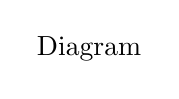
\begin{tikzpicture}
                \node {Diagram};
            \end{tikzpicture}
        \end{center}
        
    \item Which of the following statement(s) is(are) correct? \\*
        \begin{tasks}(2)
            \task $\beta = 0$ when $a = g/\sqrt{2}$
            \task $\beta > 0$ when $a = g/\sqrt{2}$
            \task $\beta = \sqrt{2}-1/\sqrt{2}$ when $a = g/2$
            \task $\beta = 1/\sqrt{2}$ when $a = g/2$
        \end{tasks}
        \begin{center}
            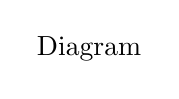
\begin{tikzpicture}
                \node {Diagram};
            \end{tikzpicture}
        \end{center}

    \item An $\alpha$-particle (mass 4 amu) and a singly charged sulfur ion (mass 32 amu) are initially at rest. They are accelerated through a potential $V$ and then allowed to pass into a region of uniform magnetic field which is normal to the velocities of the particles. Within this region, the $\alpha$-particle and the sulfur ion move in circular orbits of radii $r_{\alpha}$ and $r_{s}$, respectively. The ratio $(r_{s}/r_{\alpha})$ is \_\_\_\_\_.
    
    
\begin{enumerate}
    \item A container with 1 kg of water in it is kept in sunlight, which causes the water to get warmer than the surroundings. The average energy per unit time per unit area received due to the sunlight is 700 Wm$^{-2}$ and it is absorbed by the water over an effective area of 0.05 m$^2$. Assuming that the heat loss from the water to the surroundings is governed by Newton’s law of cooling, the difference (in $^\circ$C) in the temperature of water and the surroundings after a long time will be \underline{\hspace{3cm}}. (Ignore effect of the container, and take constant for Newton’s law of cooling = 0.001 s$^{-1}$, Heat capacity of water = 4200 J kg$^{-1}$ K$^{-1}$)
\end{enumerate}

    
    \item A small object is placed at the center of a large evacuated hollow spherical container. Assume that the container is maintained at 0 K. At time $t = 0$, the temperature of the object is 200 K. The temperature of the object becomes 100 K at $t = t_{1}$, and 50 K at $t = t_{2}$. Assume the object and the container to be ideal black bodies. The heat capacity of the object does not depend on temperature. The ratio $(t_{2}/t_{1})$ is \_\_\_\_\_.
\end{enumerate}



\pagebreak

\begin{center}
    \textsc{JEE Advanced 2022 Paper-II\\Physics\\Answer Key}
\end{center}

\begin{multicols}{4}
    \begin{enumerate}
        \item 3
        \item 2
        \item 5
        \item 4
        \item 4
        \item 3
        \item 6
        \item 3
        \item (b)
        \item (a), (b), (c)
        \item (c), (d)
        \item (a), (c), (d)
        \item (a), (b)
        \item (b), (c), (d)
        \item (b)
        \item (a)
        \item None
        \item (c)
    \end{enumerate}
\end{multicols}

\pagebreak

\begin{center}
    \textsc{JEE Advanced 2021 Paper-I\\Physics\\Answer Key}
\end{center}

\begin{multicols}{4}
    \begin{enumerate}
        \item (c)
        \item (c)
        \item (b)
        \item (d)
        \item 0.5
        \item 7.50
        \item 1.33
        \item 0.67
        \item 1.73
        \item 3.0
        \item (b), (d)
        \item (b), (c), (d)
        \item (a), (b), (c)
        \item (a), (d)
        \item (a), (c)
        \item (a), (c)
        \item 4
        \item 49
        \item 9
    \end{enumerate}
\end{multicols}

\end{document}